\chapter{Tecnologie}

\begin{figure}[hbt!]
    \centering
    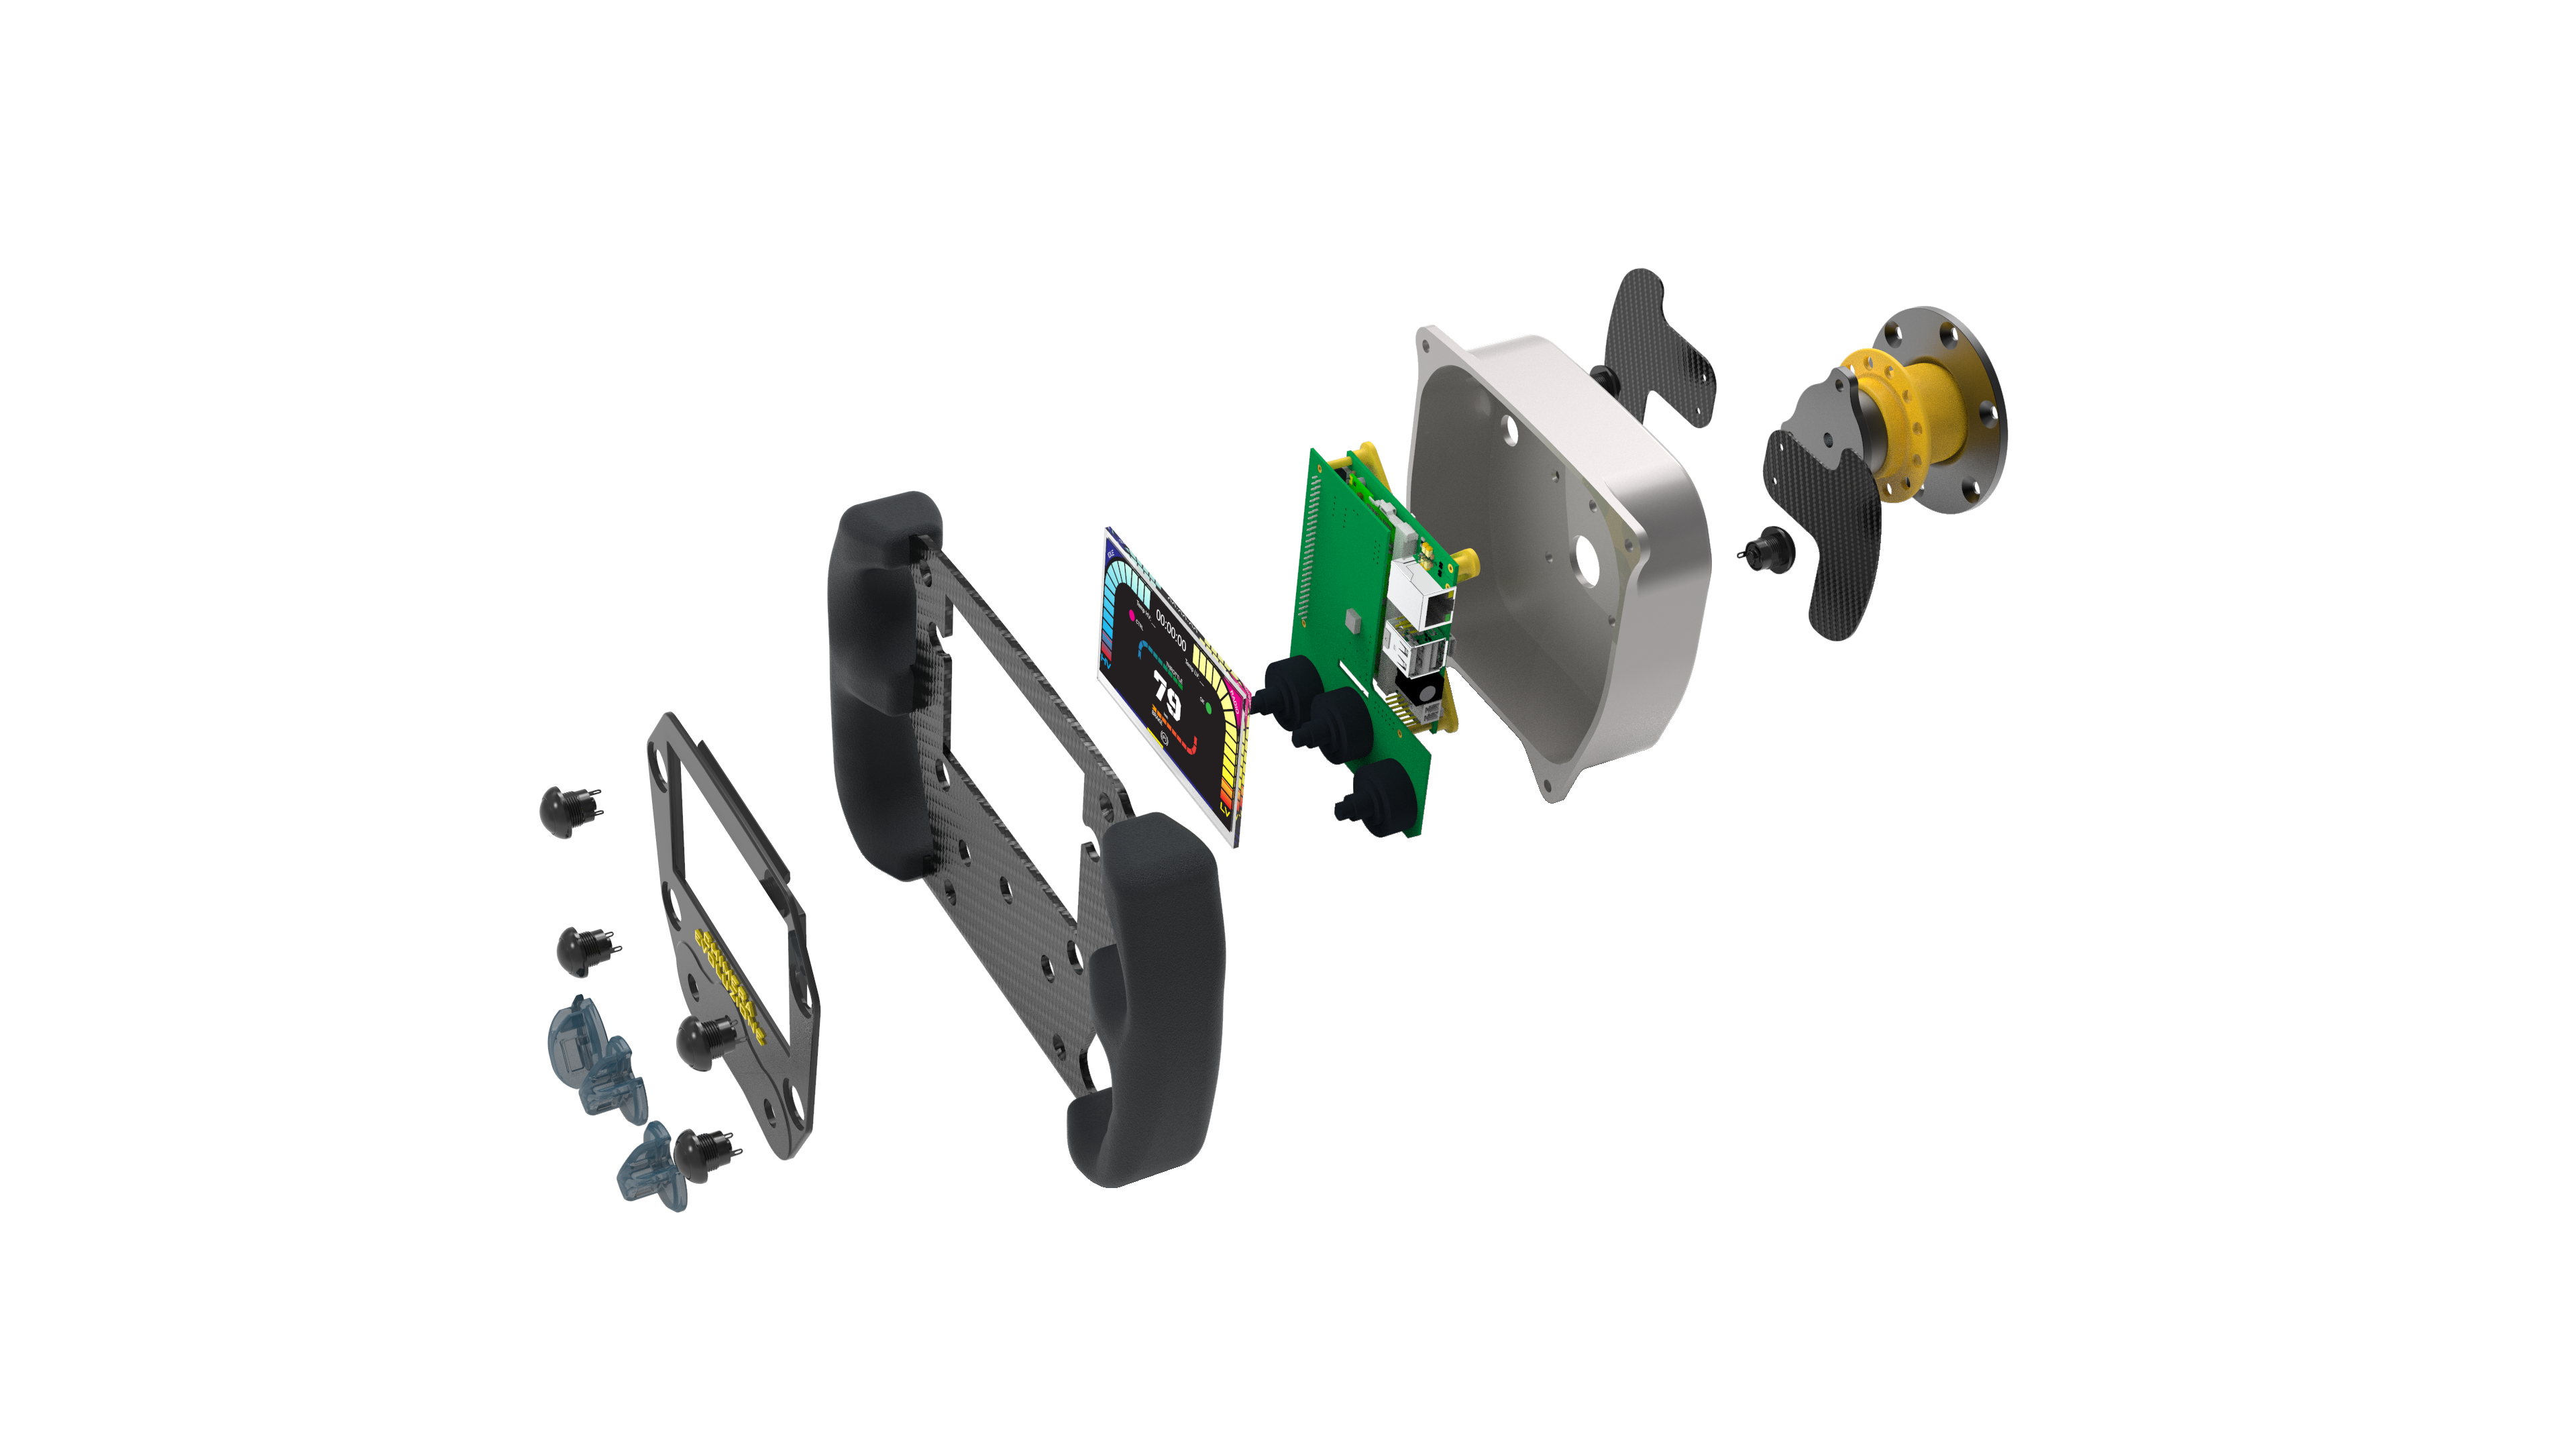
\includegraphics[width=1\textwidth]{./figures/steeringwheelEsploso.png}
    \caption{Esploso del Volante}
\end{figure}

% grazie al confronto di studenti e professori -> idee vincenti 
Durante l'intero progetto del Volante si è sempre cercato di confrontarsi con professori competenti nel settore di referimento.
Questo ha portato ad acquisire sempre più idee possibili per poter trovare soluzioni ottimali e innovative ai nostri problemi.
L'interdisciplinità del progetto ha fatto si che professori, provenienti anche da dipartimenti diversi avessero la possibilità di dare importanti 
contributi e utili consigli, su quali tecnologie potessero fare al caso nostro.
Questo ha fatto si che ogni singola scelta dovesse essere motivata e costruita da una base di esperienze personali facoltative e considerazioni
giustificate con esempi. Queste scelte sono poi state discusse in gruppo per essere approvate da tutti.
Le scelte prese sono state abbastanza indipendenti, considerando il settore meccanico e software/elettronico, considerando le limitazioni che si potrebbero affrontare.
Non si sono verificate situazioni in cui una nostra possibile scelta non potesse essere presa vedendo come ostacolo ad esempio il case del Volante.
Le difficoltà invece si sono ritrovate nel interfacciare il sistema operativo con l'hardware che, per nostra inesperienza, ha portato ad alcune 
situazioni in cui i lavori sono rallentati.   


\newpage


\section{Scelta del Hardware}

\begin{figure}[hbt!]
    \centering
    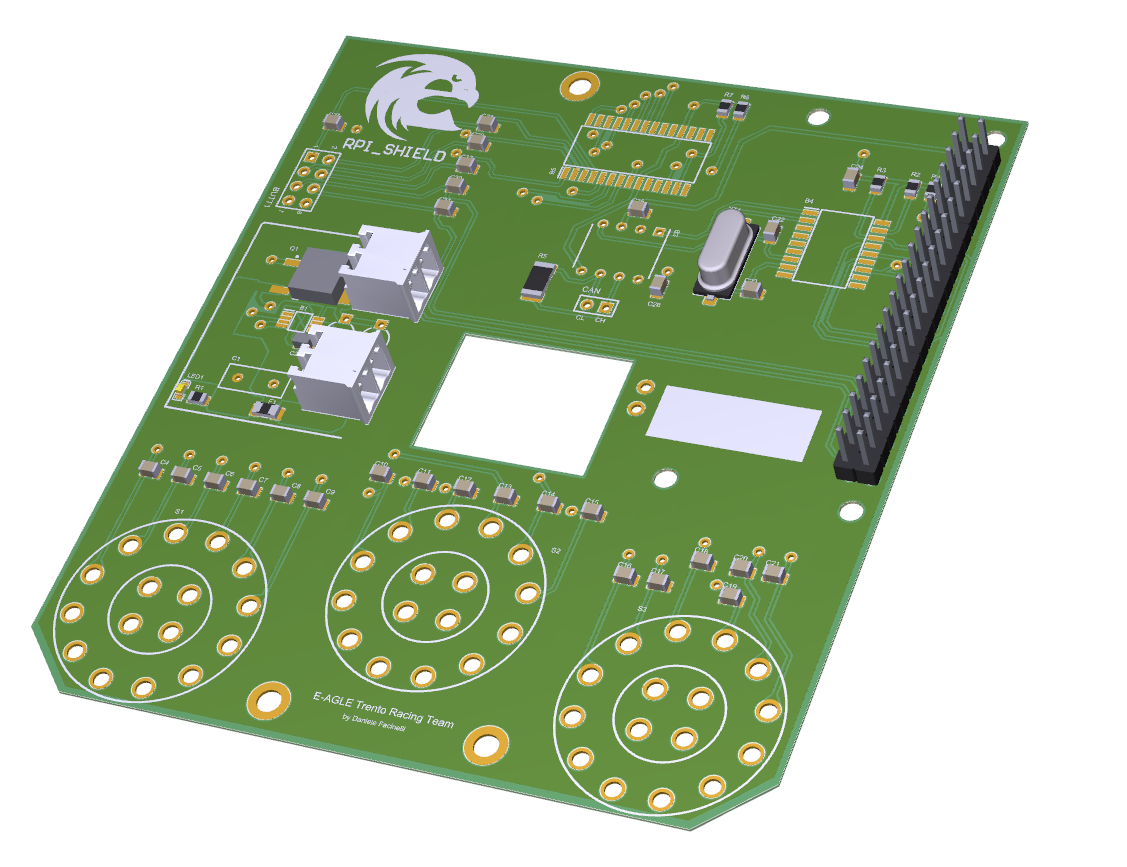
\includegraphics[width=0.75\textwidth]{./figures/imageshield.png}
    \caption{Shield del Volante}
\end{figure}

%   perchè abbiamo scelto raspberry pi zero (linux), 
%   in cosa ci ha avvantaggiato (money) (facilità di averla) (sostituirla con altre schede)
%   Funzionamento Shield

La scelta della scheda si è basata principalmente su due aspetti molto importanti, il prezzo e la facilità di sviluppo.
Dopo aver fatto ricerche per la compatibilità di diversi software l'utilizzo di un Raspberry è risultato sin da subito la scelta 
più pertinente dato il nostro backgorund di studenti appassionati di elettronica e software.
In particolare la nostra attenzione è caduta su Rasberry Pi Zero un dispositivo low cost, con la possibilità di avere una connessione 
wifi on-board (facilità di collegarsi ad AP), dimensioni e peso ridotte e adattabile a diversi dispositvi di input/output.
Raspberry vanta una community di appassionati e sviluppatori nel settore informatico molto vasta, questo ha permesso di trovare 
esempi e documentazione con facilità.
Raspberry Pi Zero può essere poi aggiornato alle versione più performanti senza troppi problemi, montando un processore ARM 
prodotto dalla casa Broadcoam, nel nostro caso (BCM2835), necessità solo di aggiustamenti software, mantenendo uguale l'ambiente software.
Ciò che rende unico il nostro Volante è il fatto di essere custom in tutte le sue parti.
Per necessità è stata disegnata una shield collegata ai GPIO del Raspberry 
per poter aumentare e utilizzare al meglio le sue funzioni di input e output.
Per quanto riguarda le interfacce di input del pilota, per poter utilizzare più tasti e più manettini (3 manettini da 6 posizioni), 
è stato introdotto sulla shield un I2C multiplexer, precedentemente utilizzando un solo manettino non era necessario.
Come display è stato scelto di utilizzare un LCD 4.3" TFT, collegato alla scheda via HDMI, grazie a un modulo di \emph{Adafruit} per poter
avere una maggiore scelta, in quanto sul mercato momentaneamente per quanto riguarda le  specifiche tecniche i display che 
escono direttamente in HDMI hanno una luminosità troppo bassa per poter essere usati sotto il sole. 
Le nostre necessità sono state, dal punto di vista del pilota, di avere quattro tasti fisici nella parte frontale 
per poter utilizzare l'interfaccia, due paddle per potersi muovere nelle diverse tab e 
tre manettini per poter gestire la configurazione della macchina.
Per quanto riguarda invece l'interfaccia di comunicazione con il resto della macchina si è reso necessario l'utilizzo del SPI
per poter comunicare in Can-Bus utilizzando l'MCP2515 e l'alimentazione, che passa per il sistema di aggancio rapido, per poter alimentare il Volante a 5V.



\newpage


\section{Scelta del Case}

\begin{figure}[hbt!]
    \centering
    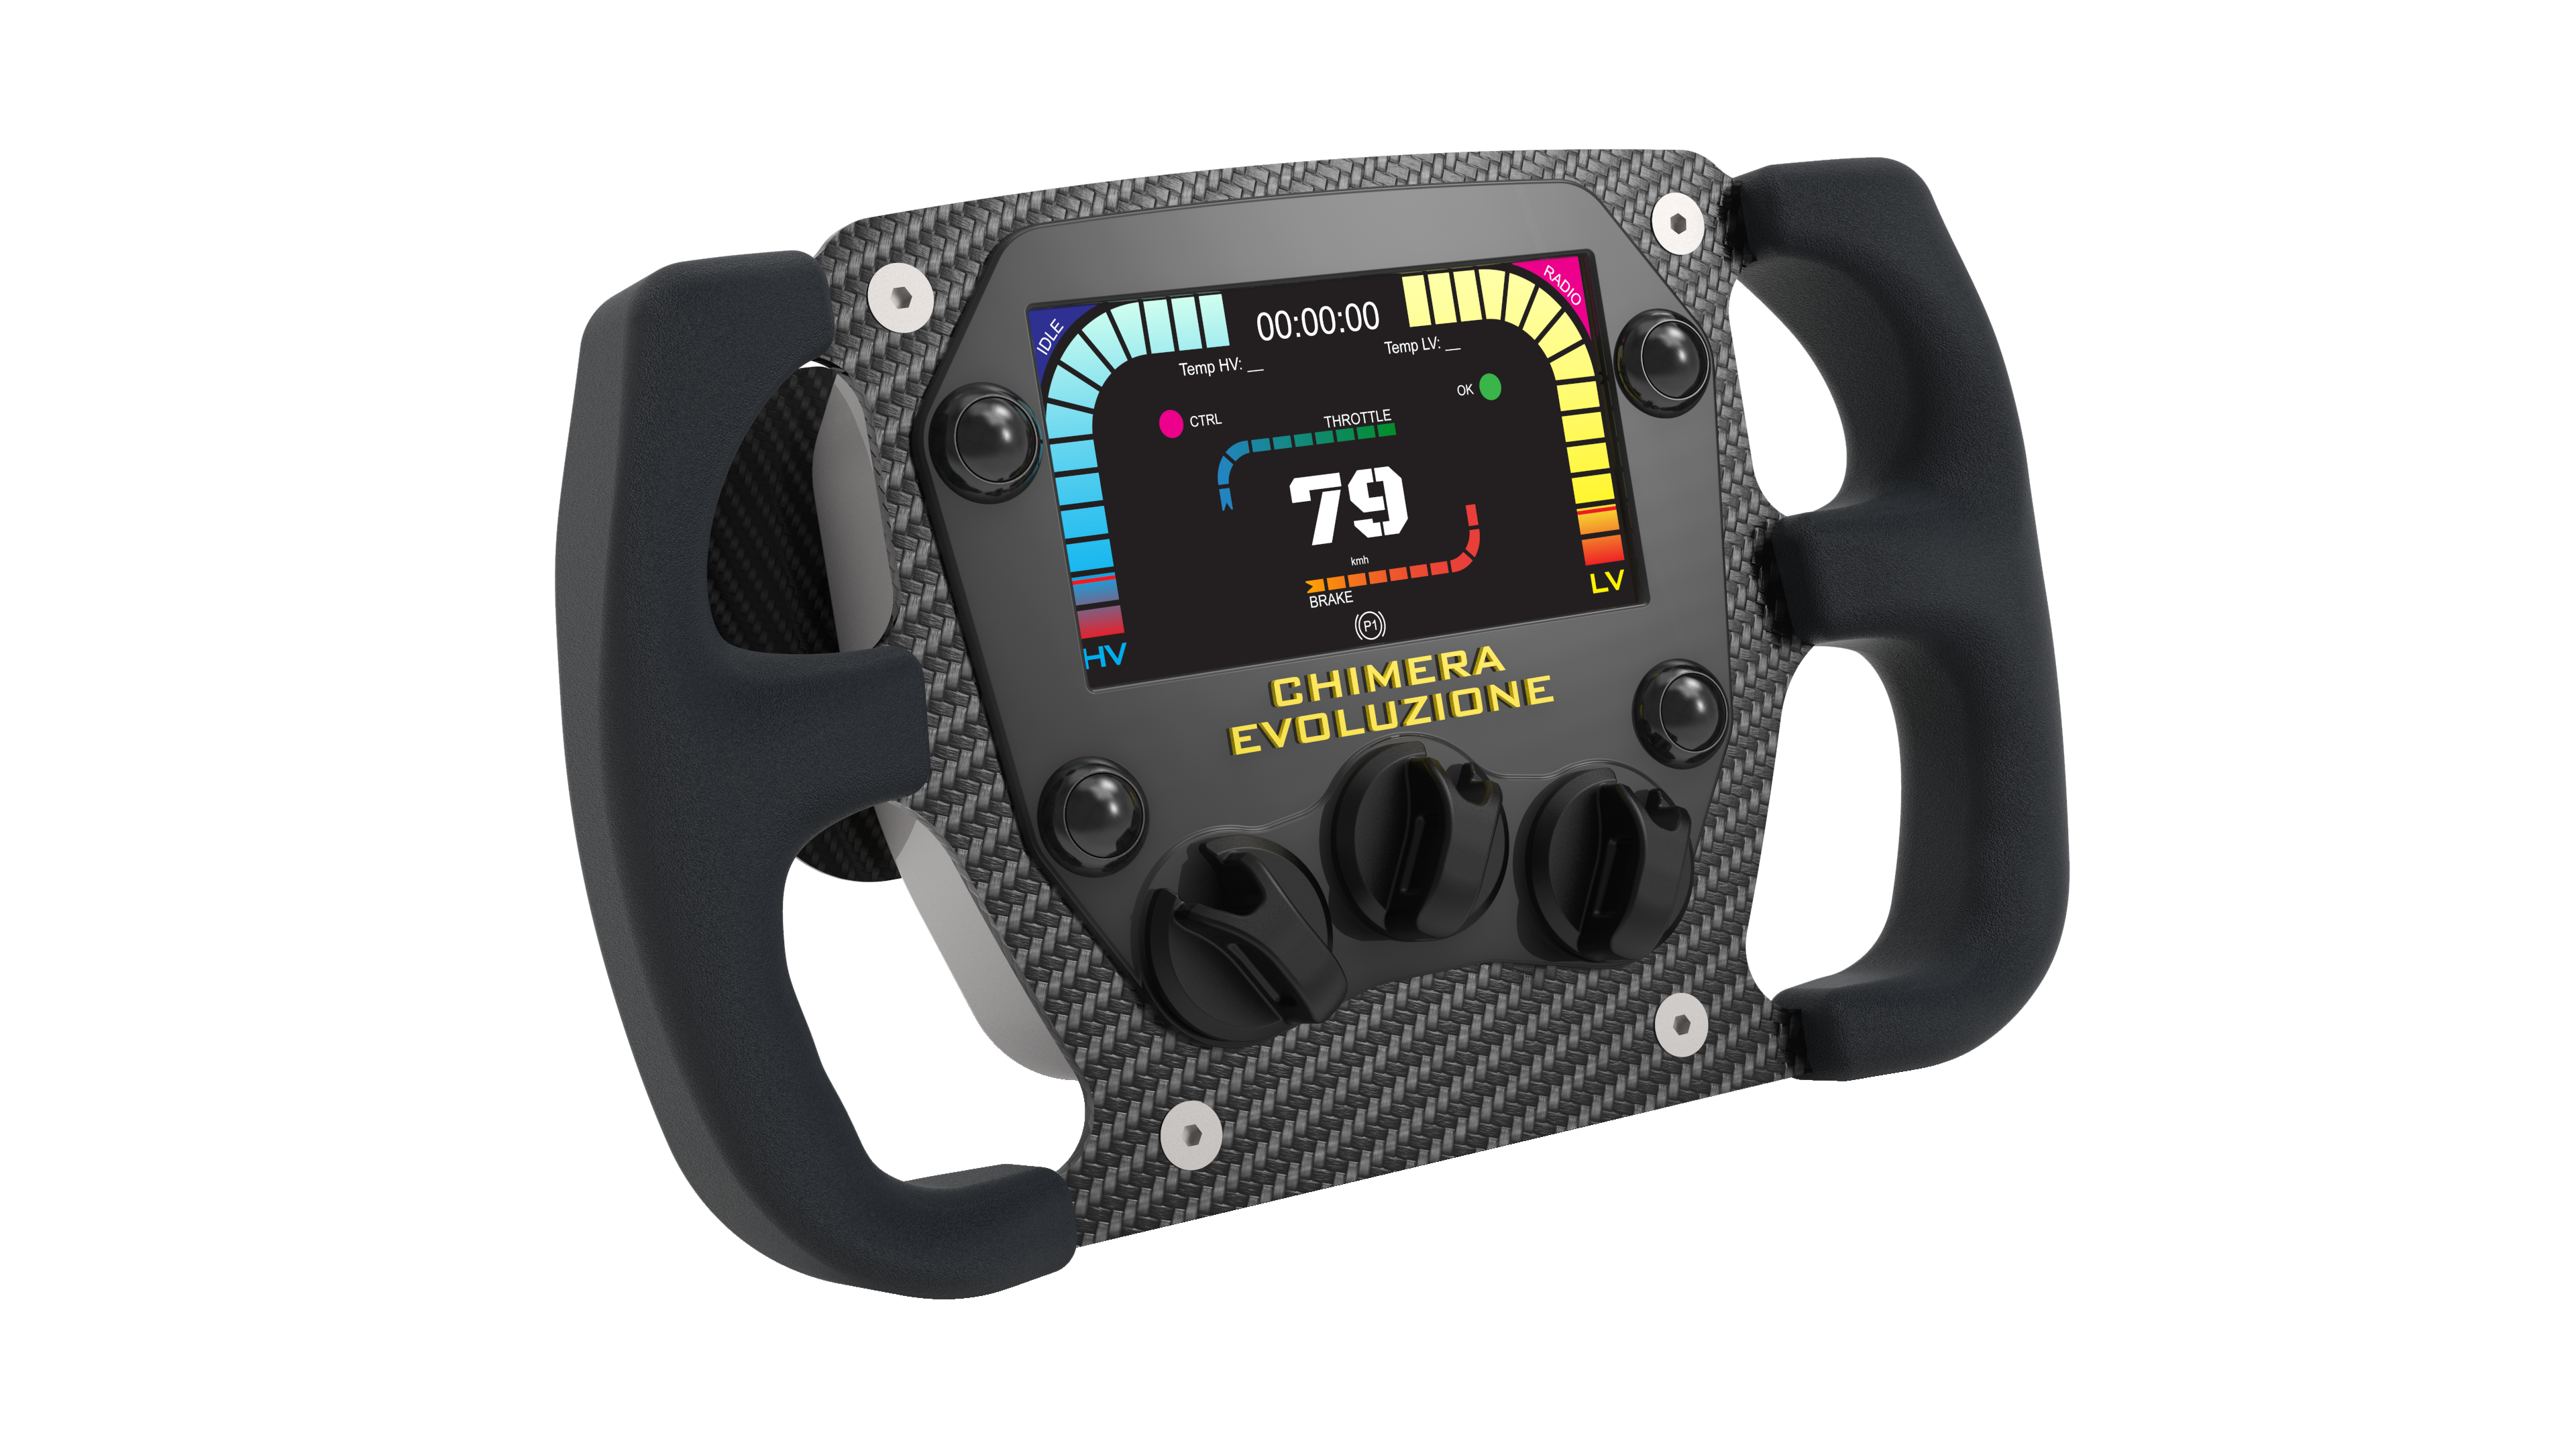
\includegraphics[width=1\textwidth]{./figures/imagemockup.png}
    \caption{Primo Mockup del Volante di Chimera Evoluzione}
\end{figure}

% Parte tradotta di Ciro e con giustificazioni sulla forma date dalla dimensione della scheda interna, costruitto attorno

La scelta di ridisegnare il case, rispetto al modello del'anno precedente 
nasce dall'esigenza di avere una maggiore ergonomia, una maggiore usabilità
e la possibilità di aggiornare le funzionalità in corso di sviluppo.
I materiali utilizzati nella versione precedente non erano adatti 
ad un uso sotto stress e non risultava facile il debug della componentistica hardware
in fase test. 
Per quanto riguarda il design del Volante di Chimera Evoluzione le scelte 
sono state prese per soddisfare il regolamento e valutando lo spazio all'interno
riservato alla componentistica elettronica.
I requisti che abbiamo considerato sono stati una maggiore robustezza, ergonomia
qualità dei materiali, facilità di assemblaggio ed estetica per venire incontro 
alle esigenze del pilota.
Per la parte di produzione è stata fatta una ricerca sulle migliori soluzioni che potevamo
utilizzare per costruirlo e con i materiali che più venivano incontro alle nostre esigenze.

Tutte le componenti sono state disegnate e realizzate dal team nei nostri laboratori.

\begin{itemize}
    \item Piastra Principale: fibra di carbonio con core interno in schiuma da 1.5 mm per uno spessore totale di 3 mm, trattamento di cura in autoclave. Rifinito con tecnologia di taglio ad acqua per ottenere la forma desiderata.
    \item Paddle: 5 strati di fibra di carbonio, Trattamento di cura in autoclave, rifinito con taglio ad acqua.
    \item Mascherina Frontale: Stampata in 3D con processo di stereolitografia, Materiale: Resina, Stampante: Form 2
    \item Manettini: MJF (Multi Jet Fusion) with HP Jet Fusion 3D 4200 printer, PA 12 powder, sandblasted and painted
    \item Imppugnatura: Stampata in 3D con processo di stereolitografia, Materiale: Resina, Stampante: Form 2. Incollati con adesivo strutturale.
    \item Guscio Posteriore: Alluminio serie aeronautica, lavorato da un blocco grezzo con fresa CNC a 5 assi
\end{itemize}


\newpage


\section{Scelta del Sistema Operativo}

\begin{figure}[h!]
    \centering
    \begin{minipage}{0.5\textwidth}
        \centering
        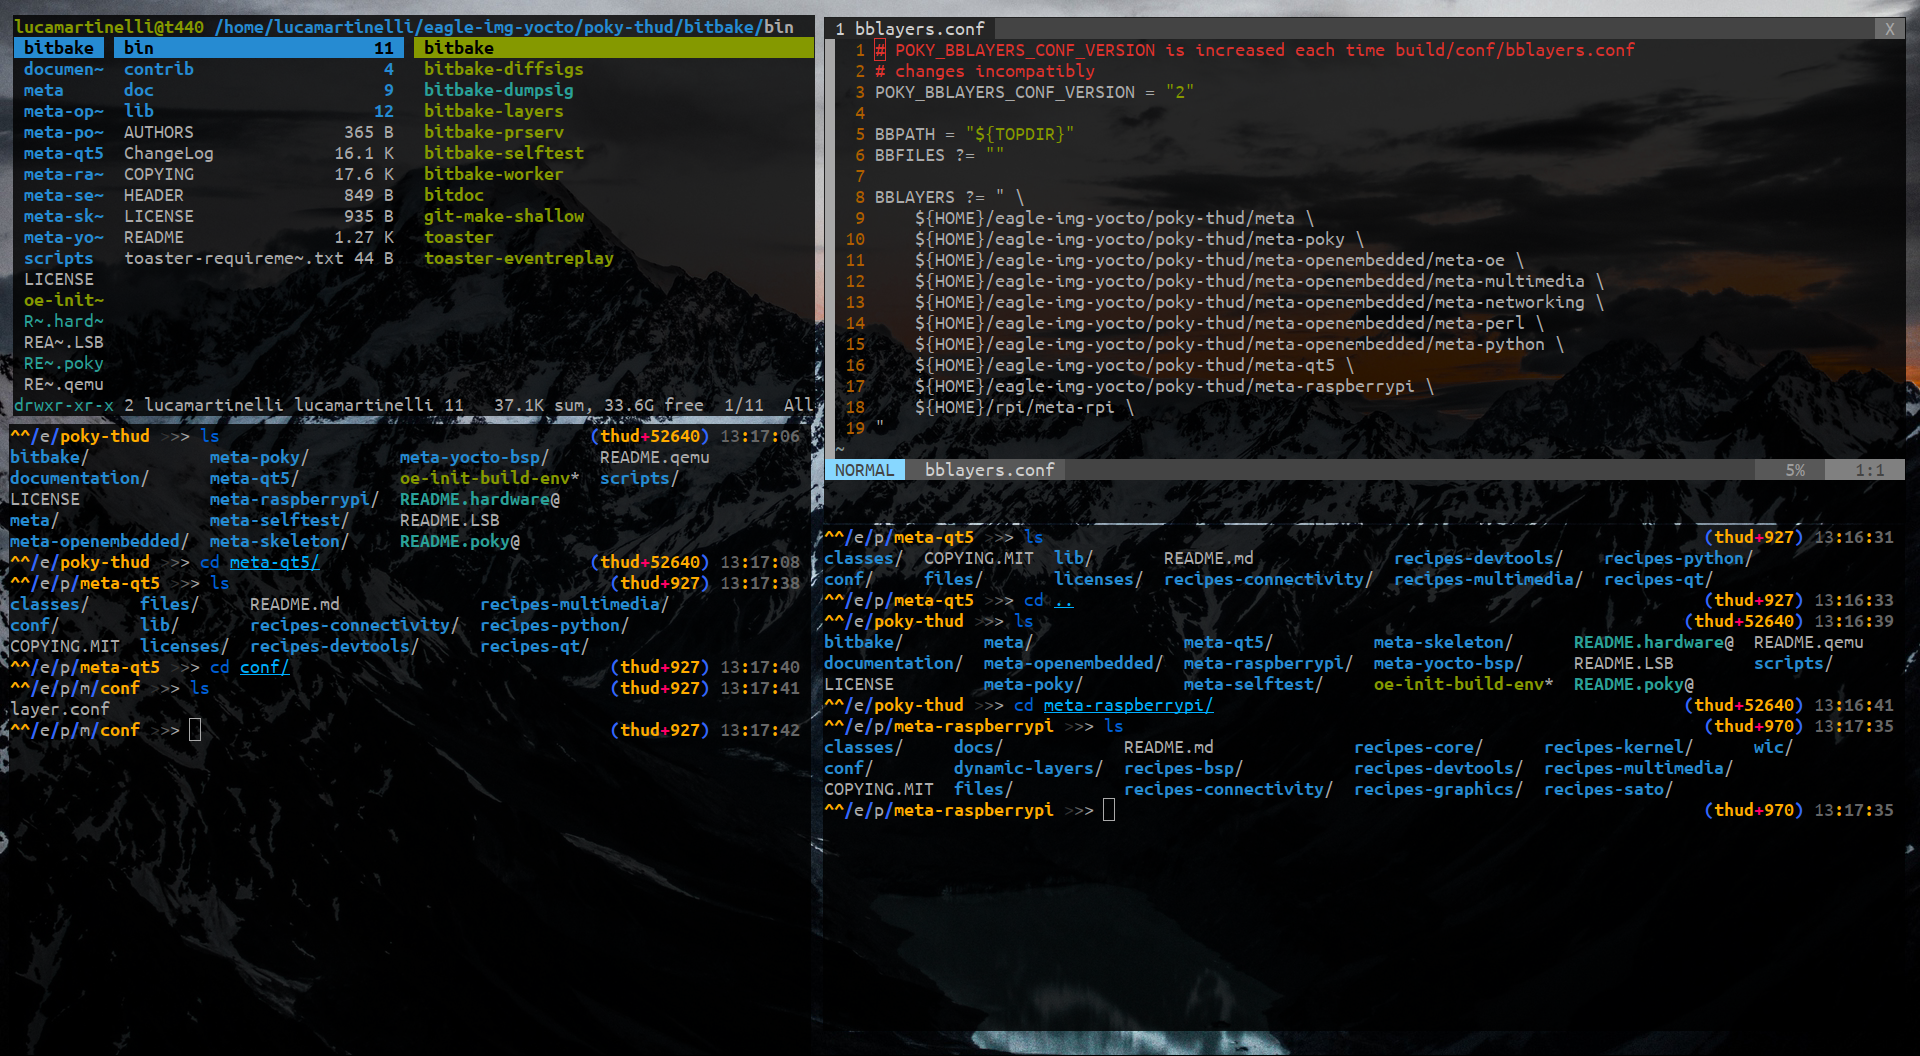
\includegraphics[width=8cm]{./figures/yoctoWorkFlow.png} % first figure itself
        \caption{Yocto preparazione dell'ambiente}    
    \end{minipage}\hfill
    \begin{minipage}{0.5\textwidth}
        \centering
        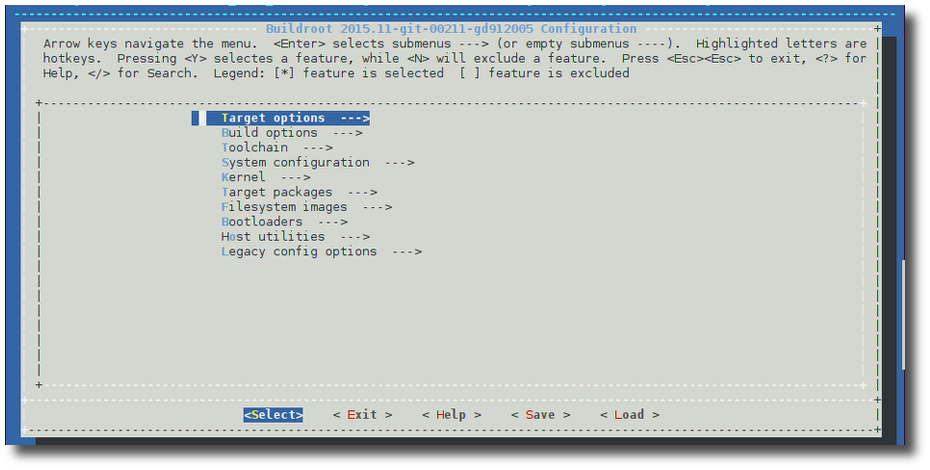
\includegraphics[width=8cm]{./figures/menuBuildRoot.png} % second figure itself
        \caption{Builroot - Primi passi della fase di build}        
    \end{minipage}
\end{figure}

% debug di linux e facilità di implementare funzionalità in breve tempo 

La scelta della scheda ci ha portato ad utilizzare in fase di test una delle ultime
versioni stretch di Raspbian presenti nel 2017. Le ottimizzazioni sono state in termini
di boot time, l'autostart della applicazione, la connesione a reti wireless,
la configurazione dell'uscita hdmi per il display e le librerie necessarie per poter eseguire il programma. 
I nostri requisiti sono stati principalmente due, il poter compilare senza dover utilizzare il Volante,
lasciando così il dispositivo il più leggero possibile e poterlo utilizzare come sistema di debug della macchina.
L'utilizzo di \emph{SocketCan}, attraverso il paccheto \emph{can-utils} ci ha permesso in più situazioni di gestire e leggere i messaggi
senza eseguire il software del Volante, ma come una macchina linux collegata ad essa via \emph{ssh} e per aggiornare il codice via \emph{scp}.
Una volta definiti tutti i requisiti e attraverso il progetto open-source \emph{buildroot} abbiamo sviluppato
un sistema operativo con tutte le specifiche richieste, successivamente le condizioni sono cambiate e
abbiamo deciso di spostarci verso un altro ambiente di cui è presente più documentazione che spiegherò nel prossimo sottocapitolo. 
Grazie alla diversificazione delle ricette è possibile aggiornare la componentistica hardware cambiando alcuni parametri 
prima della fase di build, questo ci ha permesso di mantenere una buona stabilità nel workflow senza dover mantenere più progetti, ma 
solamente di modificare la ricetta di quello già esistente e integrare i pacchetti necessari per la scheda di riferimento.
Mantenere lo stack di un sistema operativo Linux ha permesso di integrare facilemente le funzionalità dalla versione
desktop a quella in macchina, soprattutto per la cross-compilazione.
Durante il secondo semestre del 2018 per necessità del team mi è stato chiesto di verificare alcune soluzioni per poter avere un sistema operativo
\emph{"real-time"}, tra le possibilità la più interessante sulla quale ho fatto alcuni test e ricerche è risultata essere \emph{Xenomai}, ma per 
mancanza di tempo e sviluppatori il progetto è stato abbandonanto dovendo concludere lo sviluppo del Volante per Chimera Evoluzione.
Successivamente, grazie ai risultati ottenuti con il Volante, questo non è risultato più un problema avendo altre alternative più facili da implementare.

\newpage

\section{Scelta del Framework}

\begin{figure}[h!]
    \centering
    \begin{minipage}{0.5\textwidth}
        \centering
        
\includegraphics[width=8cm]{./figures/qtIcon.jpg} % first figure itself
    \end{minipage}\hfill
    \begin{minipage}{0.5\textwidth}
        \centering
        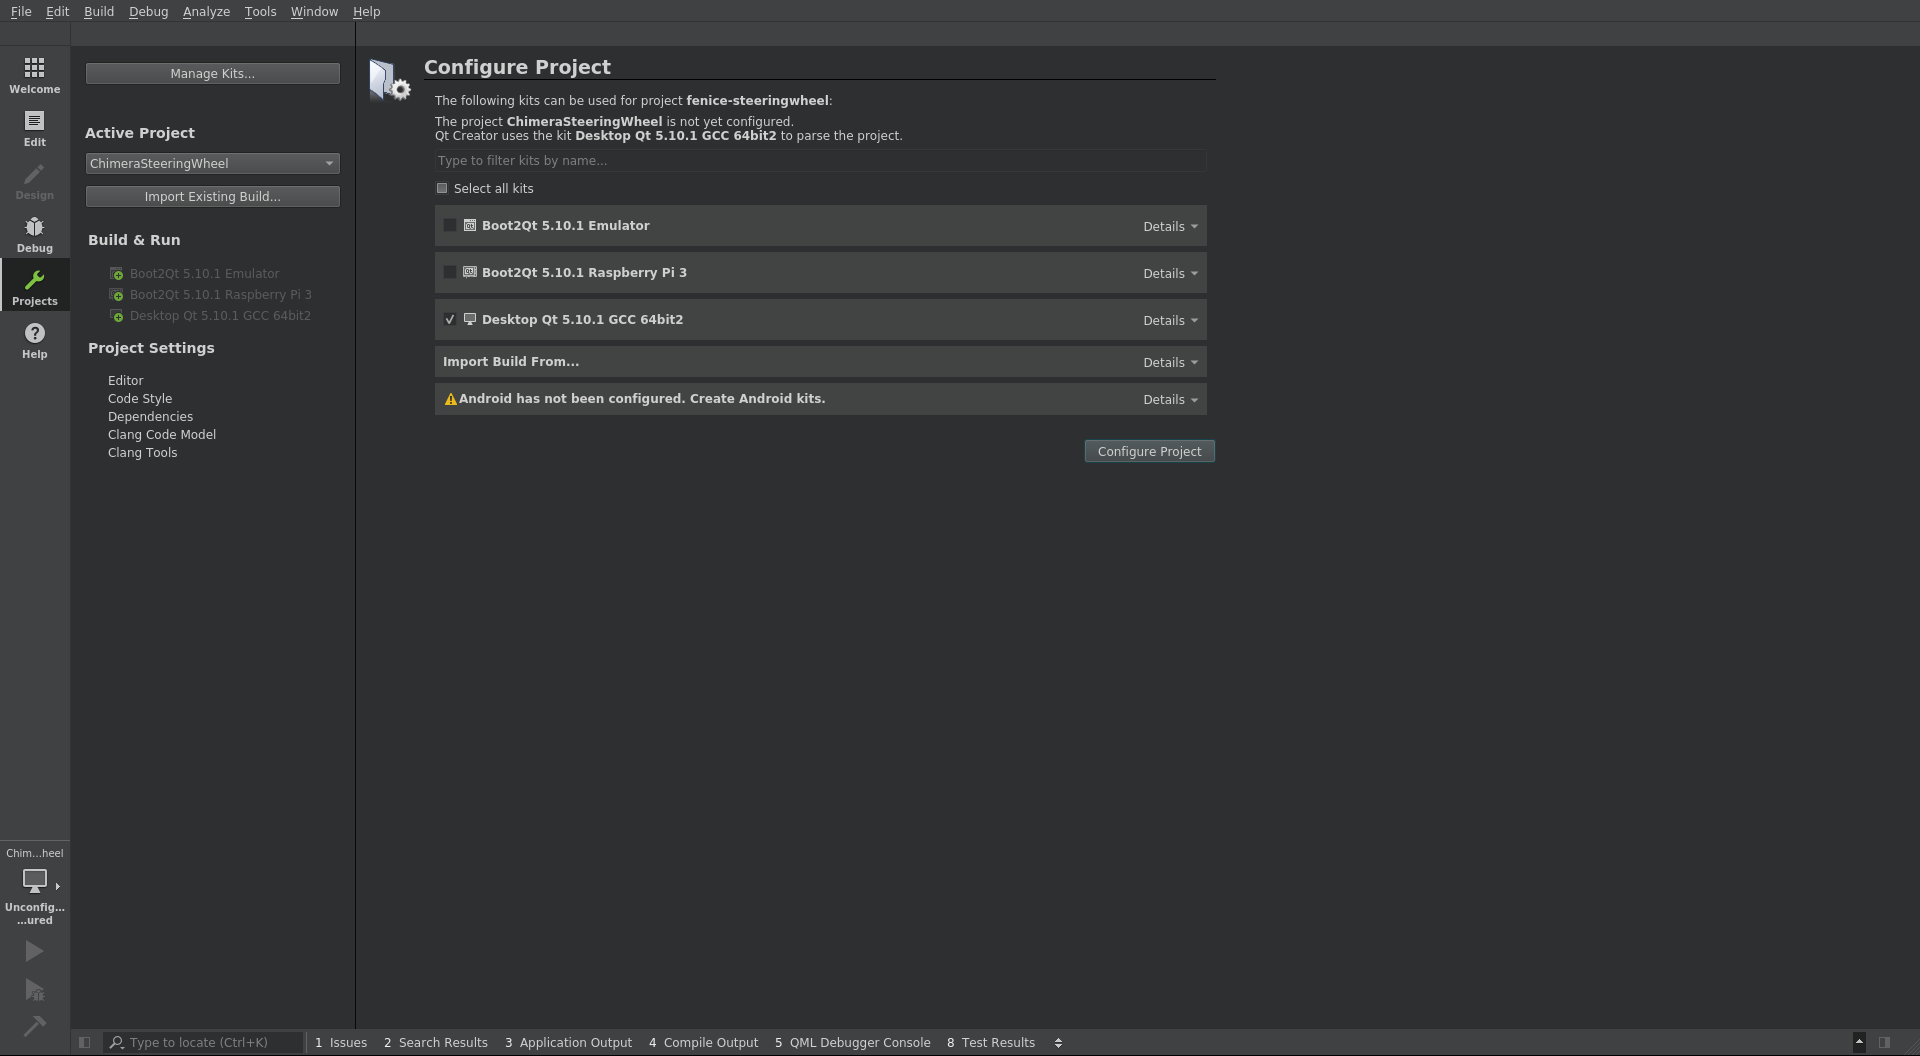
\includegraphics[width=8cm]{./figures/qtCreator.png} % second figure itself
        \caption{Qt Creator - apertura di un progetto e scelta del compilatore}                
    \end{minipage}
\end{figure}

%   perchè abbiamo scelto qt (buona base di partenza) e comodità di questo framework (compatibilità, multipiattaforma)
%   Discorso di sponsorizzazione e di conseguenza facilità di utilizzare i loro pacchetti con yocto

La scelta del framework era già stata fatta precedentemente il mio arrivo nel team, la decisione 
che è stata presa per Chimera Evoluzione è stata quella di voler terminare il lavoro dell'anno precedente 
aggiornarlo e renderlo il più possibile stabile e adatto alle nostre esigenze.
Il framework in considerazione risulta essere Qt, che permette grazie alle sue librerie grafiche 
multipiattaforma di lavorare in C++ e disegnare in breve tempo interfacce grafiche.
Qt, oltre ad essere utilizzato per soluzioni embedded, vanta numerosi esempi nel campo dell'automotive, è infatti 
presente nelle dash digitali di alcuni modelli nel mercato automobilistico.
I vantaggi di questo framework sono la diversificazione del lavoro in termini di sviluppo, chi si occupa 
di aggiornare la parte grafica, quindi il FE, non per forza deve essere in stretta relazione con chi sviluppa la parte
di backend del progetto, garantendo un workflow più dinamico. 
Qt nasce come framework open-source, i progetti che abbiamo preso in mano per capirne le potenzialità erano
sviluppati su Raspberry o comunque sistemi Linux e facilmente portabili a piattaforme embedded, non tanto per 
la parte di compilazione ma del progetto in senso stretto.
Inoltre Qt risulta abbastanza intuitivo al primo approccio utilizzando la sintassi di C++ ma, le prime difficoltà 
si riscontrano nell'utilizzare le funzioni proprietarie che, anche se fornite con una buona documentazione, non sempre
risulta completa.

Questo framework presenta anche una versione commerciale distribuita da \emph{The Qt Company}, 
con la possibilità di utilizzare \emph{tool} proprietari disegnati per facilitare il lavoro degli sviluppatori e ampliarne le funzionalità  
attraverso ulteriori librerie e pacchetti per compilare su dispositivi embedded.
Oltre alla community, che presenta sempre discussioni interessanti sulle nuove funzionalità implementate, con la versione commerciale
si ha a disposizione un servizio di assistenza e consulenza.    

L'accesso ai GPIO è stato gestito utilizzando le librerie di \emph{wiringpi} \cite{wiringPI} che, oltre a permetterci di gestire i singoli bottoni,
ci ha permesso grazie al multiplexer di leggere lo stato dei diversi encoder utilizzati come manettini. 

Nel Settembre 2018, dopo i risultati ottenuti durante la stagione, ci siamo proposti a \emph{The Qt Company} per avere una sponsorizzazione.
Questo ci ha permesso di mettere in relazione l'Università degli Studi di Trento con l'azienda e ampliare la rete dei legami del progetto.
Inoltre ha avuto un impatto positivo per il nostro workflow, avere a disposizione le funzionalità complele del framework ci ha permesso di
usare l'immagine stock di Qt per Raspberry per la parte di test e la loro \emph{compile-tool} per dispositivi embedded presente nel pacchetto \emph{boot2qt}
Nel paccheto è presente inoltre una guida basata sui tool di \emph{Yocto}, in particolare la versione \emph{Poky}, per poter costruire da zero 
una versione base per supportare la applicazioni embedded, per questo ho deciso di abbandonare l'utilizzo di \emph{Buildroot}, in favore di una maggiore 
documentazione \cite{jumpnowtek}. 
   
  
\newpage